
% !TeX root = RJwrapper.tex

\title{Refreg: An R Package for Estimating Conditional Reference Regions}
\author{by Lado-Baleato, Óscar, Roca-Pardiñas, Javier, Cadarso-Suárez, Carmen and Gude, Francisco}

\maketitle

\abstract{Multivariate reference regions (MVR) represent the extension of the reference interval concept to the multivariate setting. A reference interval is defined by two threshold points between which a high percentage of healthy subjects’ results, usually 95\%, are contained. Analogously, an MVR characterizes the values of several diagnostic tests most frequently found among non-diseased subjects by defining a convex hull containing 95\% of the results. MVRs have great applicability when working with diseases that are diagnosed via more than one continuous test, e.g.,  diabetes or hypothyroidism. The present work introduces \pkg{refreg}, an R package for estimating conditional MVRs. The reference region is non-parametrically estimated using a multivariate kernel density estimator, and its shape allowed to change under the influence of covariates. The effects of covariates on the multivariate variable means, and on their variance-covariance matrix, are estimated by flexible additive predictors. Continuous  covariate non-linear effects can be estimated by penalized spline smoothers. The package allows the user to propose, for instance, an age-specific diagnostic rule based on the joint distribution of two non-Gaussian, continuous test results. The usefulness of the \pkg{refreg} package in clinical practice is illustrated with a real case in diabetes research, with an age-specific reference region proposed for the joint interpretation of two glycemia markers (fasting plasma glucose and glycated hemoglobin). To show that the \pkg{refreg} package can also be used in other, and indeed very different fields, an example is provided for the joint prediction of two atmospheric pollutants (SO$_2$, and NO$_x$). Additionally, the text discusses how, conceptually, this method could be extended to more than two dimensions.}
	
\section{Introduction}

In clinical practice, many medical decisions are based on continuous diagnostic tests \citep{hallworth201170} – i.e., tests that provide results along a continuous, quantitative scale. The interpretation of such continuous tests requires the comparison of the obtained value with a pre-defined reference interval, so that a result could be classified as positive or negative (ie, disease present or absent) based on this comparator value. A reference interval is an interval containing most healthy subjects’ results. For a single test they are usually estimated from the 2.5 and 97.5 empirical percentiles of the distribution for the healthy population; thus, 95\% of healthy patients are located within the interval limits \citep{wright1999calculating}. Those patients falling outside the reference interval, are likely to have an undiagnosed disease. If the test results are influenced by some patient characteristics independent of the disease (e.g., age and gender), reference intervals for specific patient groups must be obtained. These covariate-dependent reference intervals, usually termed reference curves, are estimated using quantile regression \citep{koenker1978regression} or location-scale models \citep{cole1992smoothing,stasinopoulos2017flexible}. Several R packages for estimating reference intervals and reference curves already exist, including the R package  \CRANpkg{referenceIntervals}, which comprises a collection of tools, the R package \CRANpkg{gamlss} \citep{stasinopoulos2007generalized}, which provides a general tool for deriving reference curves in clinical practice  \citep{who_gamlss}, and software \textit{RefCurv} \citep{winkler2019refcurv}, recently proposed to facilitate clinicians' use of \CRANpkg{gamlss}. However, all these packages were produced to provide reference intervals for single tests; they cannot address diseases for which diagnosis and control are based on multiple tests.

%In clinical practice, many medical decisions are based on continuous diagnostic tests \citep{hallworth201170}, the interpretation of which requires a reference interval, i.e., one that characterizes healthy subjects' results. Reference intervals for a single test are estimated from the 2.5 and 97.5 empirical percentiles of the distribution for the healthy population; thus, 95\% of healthy patients are located within the interval limits \citep{wright1999calculating}. If the test results are influenced by some patient characteristics independent of the disease (e.g., age and gender), the reference intervals for specific patient groups must be obtained. These covariate-dependent reference intervals, usually termed reference curves, are estimated using quantile regression \citep{koenker1978regression} or location-scale models \citep{cole1992smoothing,stasinopoulos2017flexible}. Several R packages for estimating reference intervals and reference curves already exist, including the R package  \CRANpkg{referenceIntervals}, which comprises a collection of tools, the R package \CRANpkg{gamlss} \citep{stasinopoulos2007generalized}, which provides a general tool for deriving reference curves in clinical practice  \citep{who_gamlss}, and software \pkg{RefCurv} \citep{winkler2019refcurv}, recently proposed to facilitate clinicians' use of \CRANpkg{gamlss}. However, all these packages were produced to provide reference intervals for single tests; they cannot address diseases for which diagnosis and control are based on multiple tests.

When the results of several tests are available for the same patient, obtaining separate reference intervals for each one provides an incomplete picture of disease status, particularly when these results are strongly correlated \citep{boyd2004reference}. Although each reference interval would leave only 5\% of healthy patients out, their combined use can result in a higher percentage of false positives. Moreover, a patient falling within each univariate reference interval might, in fact, show an abnormal multivariate result. Thus, a multivariate reference region (MVRs) would provide a better means of interpreting the results of multiple tests \citep{winkel1972normal}. MVRs are a straightforward extension of the univariate reference interval to the multidimensional setting, i.e., a region that contains 95\% of the healthy patients' results. However, despite being proposed more than 40 years ago, MVRs are rarely used in clinical practice. This might be explained by the multivariate Gaussian assumption of MVRs, which is quite restrictive when interpreting diagnostic test results. Further, the multivariate distribution of test results is usually affected by patient characteristics, independent of their health status. For example, \cite{espasandin2019assessing} showed that the correlation between two diagnostic tests for diabetes was influenced by patient age and red blood cell turnover, independent of glycemia status. A conditional MVR is therefore desirable, but the statistical literature is not rich in such proposals (see, e.g., \citep{wei2008approach}).

Very few statistical software routines have been proposed for estimating the region containing a specific percentage of multivariate data points. The function \code{mvtol.region} in the R package \CRANpkg{tolerance} \citep{young2010tolerance} obtains a region containing a high percentage of a bivariate Gaussian distribution in the context of quality control studies, and non-parametric probabilistic regions can be obtained using the R packages \CRANpkg{r2d2} \citep{r2d2}, \CRANpkg{hdrcde} \citep{hdrcde} and  \CRANpkg{distfree.cr} \citep{distfree}. However, these all suffer the major limitation of not being able to estimate the effects of covariates on the region’s shape. The R package \CRANpkg{modQR} can estimate conditional multivariate quantiles, but the quantile level $\tau$ is not linked to the probability content of the sample \citep{siman}. Thus, it is not clear how to derive a reference region from these bivariate quantiles.

The present paper introduces \pkg{refreg}, an implementation in R of a new statistical methodology for estimating bivariate reference regions able to classify subjects as having normal or abnormal values based on the results of two continuous diagnostic tests. The main advantages of the presented method are; i) the absence of parametric restrictions for describing bivariate distributions for continuous tests, and ii) the possibility of estimating the effects of covariates on the shape of the reference region via flexible additive predictors. To illustrate this statistical methodology, and how to use the package, an age-specific reference region for two diabetes diagnostic tests was estimated. The estimated reference region offers new insights into the diagnosis and prognosis of diabetes, enabling physicians to identify different patients’ profiles. The proposed method can, however, be applied to any disease in which two continuous diagnostic tests are available, and can even be used in non-medical fields. Indeed, an application is discussed in which the conditional region is used in the joint forecasting of the concentrations of two air pollutants. Moreover, the current implementation can be easily extended to three dimensions.

The statistical model that enables conditional reference regions to be determined is presented in the next section. The main functions contained in the \pkg{refreg} package are then described, with a brief introduction to the main functions. The use of the package is shown in analyses of real medical and environmental data problems. The paper closes with some comments, and some notes on future research directions.

\section{Statistical methodology}

In this section the main features of our statistical method is presented. In a nutshell, our proposal is based on a bivariate location scale model, where the response means, and their variance-covariance matrix, are related to covariates using flexible additive predictors. The probabilistic region covering a specific percentage of the data is firstly estimated using the model standardized residuals. Then, it is generalized for each covariate value based on the  aforementioned bivariate location-scale model fit. This statistical model was already presented and evaluated in \citep{roca2020nonparametric}.

\subsection{Conditional reference region}

Given a bivariate continuous random variable of interest ${\bf Y} = (Y_1, Y_2)$, and a vector of covariates $\bf{X}=(X_1, \ldots, X_p)$ we consider the following structure:
\begin{equation}
\left( {
	\begin{tabular} {c}
	$Y_1$ \\
	$Y_2$\
	\end{tabular}
}\right) = \left( {
	\begin{tabular} {c}
	$\mu_1(\textbf{X})$ \\
	$\mu_2(\textbf{X})$\
	\end{tabular}
}\right)
+  \boldsymbol{\Sigma}^{1/2} (\textbf{X})
\left( {
	\begin{tabular} {c}
	$\varepsilon_1$ \\
	$\varepsilon_2$\\
	\end{tabular}
}\right)
\label{modelo}
\end{equation}


\noindent
where $\mu_1(\textbf{X})$ and $\mu_2(\textbf{X})$ represents the conditional means of both responses and $\boldsymbol{\Sigma}^{1/2} (\textbf{X})$ the Cholesky decomposition of the variance-covariance matrix
\begin{equation}
\boldsymbol{\Sigma} (\textbf{X})=\left({
	\begin{tabular} {cc}
	$\sigma_1^2 (\textbf{X})$  &  $ \sigma_{12} (\textbf{X})$\\
	$\sigma_{12} (\textbf{X})$ & $\sigma_2^2 (\textbf{X})$  \\
	\end{tabular}}\right)
\label{mod1}
\end{equation}
\noindent
so that $\text{Var} (\bf Y|\textbf{X})=\boldsymbol{\Sigma} (\textbf{X})=
\boldsymbol{\Sigma}^{1/2} (\textbf{X})\left({\boldsymbol{\Sigma}^{1/2} (\textbf{X})}\right)^T$. In order to guarantee the model identification (\ref{modelo}), the bivariate residuals $(\varepsilon_1,\varepsilon_2)$ are assumed to be independent of the covariates, with zero mean, unit variance, and zero correlation. 


We consider additive structures for the mean functions $\mu_j({\bf X})$, variance functions $\sigma_j^2({\bf X})$ ($j=1,2$) and the correlation function $\rho({\bf X})$ -- note that $\sigma_{12} (\textbf{X})= \hat \sigma_1(\textbf{X}) \hat \sigma_{2} (\textbf{X}) \hat \rho (\textbf{X})$. These structures are given, respectively, by 
\[
\mu_r({\bf X})=\alpha_r + \sum_{j=1}^p{f_{jr}(X_j)}, \quad
\sigma_r^2({\bf X})=H_\sigma\left({\beta_r+ \sum_{j=1}^p{g_{jr}(X_j)}}\right) \quad \text{for } r=1,2
\]
\noindent
and 
\[
\rho({\bf X}) =H_\rho \left({\gamma+ \sum_{j=1}^p{m_{j}(X_j)}}\right)
\]
\noindent
where $\alpha$, $\beta$ and $\gamma$ are parametric coefficients and  $f_{jr}$,  $g_{jr}$ and $m_j$  for $j = 1,\cdots,p$ and $r=1,2$ are smooth and unknown functions. $H_\sigma (\cdot)=\exp(\cdot)$ and  $H_\rho(\cdot)=\tanh(\cdot)$ are link functions used in the variance and correlation structures, respectively, to ensure that the restrictions on the parameter spaces ($\sigma_r^2({\bf X}) \geq 0$ and $0\leq \rho({\bf X}) \leq 1) $ are maintained. 

Based on the model presented in equation (\ref{modelo}), for a given $\textbf{X}$ the conditional $\tau^{th}$- reference region for  $(Y_1, Y_2)$ is given by:
\begin{equation}
R_{\tau}(\textbf{X})
=
\left( {
	\begin{tabular} {c}
	$\mu_1(\textbf{X})$ \\
	$\mu_2(\textbf{X})$\
	\end{tabular}
}\right)
+ 
\boldsymbol{\Sigma}^{1/2} (\textbf{X}) \varepsilon_{\tau}
\label{rexion_x}
\end{equation} 
\noindent where $\varepsilon_{\tau}$ is the unconditionally probabilistic region for the errors $(\varepsilon_1,\varepsilon_2)$ as 
\begin{equation}
\varepsilon_{\tau} (k) = \{(\varepsilon_1,\varepsilon_2) \in{R}^2 | f(\varepsilon_1,\varepsilon_2) \leq k\}
\label{rexion1}
\end{equation}
\noindent
$f$ being the density function of the bivariate residuals  $(\varepsilon_1,\varepsilon_2)$ and  $k$ is the $\tau-$quantile of $f(\varepsilon_1,\varepsilon_2)$. 


\subsection{Estimation algorithm}

In this section, we present the estimation procedure of the conditioned bivariate uncertainty region given in equation (\ref{rexion_x}). Our approach is based on the estimation of the covariate effects on the response means using an additive model, and then on the variance-covariance matrix using the squared residuals of the former models. Finally, the bivariate region $R_{\tau}(\textbf{X})$ is obtained with a bivariate kernel estimation of the standardized bivariate residuals. 

The steps of  the proposed estimation algorithm are the following:

\noindent
\textbf{Step 1:} For $r=1,2$ fit an additive model to the sample $\{{\bf X}_i, {\bf Y}_{ir}\}_{i=1}^n$ and obtain the estimates
\begin{equation}
\hat \mu_{r}({ \bf X}_i)=\hat \alpha+ \sum_{j=1}^p \hat f_{jr}(X_{ij}) 
\label{am1}
\end{equation}
\noindent
Then,  estimate $\sigma_{r}^2(\textbf{X})$  from the sample $\{{\bf X_i}, ({\bf Y}_{ir} - \hat \mu_r({\bf X}_i))^2\}_{i=1}^n$ as 
\begin{equation}
\hat \sigma_{r}^2(\textbf{X}_i)= \hat \beta_r + \sum_{j=1}^p \hat g_{jr}(X_{ij})
\label{am2}
\end{equation}
\noindent
\textbf{Step 2:} Compute the correlation $\rho (\textbf{X})$, using the sample $\{{\bf X}_i, \hat{\delta}_i\}_{i=1}^n$,  as
\[
\hat \rho (\textbf{X}_i)= \tanh \left( {\hat \gamma + \sum_{j=1}^p \hat m_{jr}(X_{ij})}\right)
\]
\noindent
where 
\[
\hat{\delta}_i = 
\frac{\left(
	Y_{i1}-\hat{\mu}_1(\textbf{X}_i)\right)\left(Y_{i2}-\hat{\mu}_2(\textbf{X}_i)
	\right)}{\hat{\sigma}_1(\textbf{X}_i)\hat{\sigma}_2(\textbf{X}_i)}
\]
\noindent
\textbf{Step 3:} Compute the standardized residuals 
\begin{equation}
\left({
	\begin{tabular} {c}
	$\hat{\varepsilon}_{i1}$ \\
	$\hat{\varepsilon}_{i2}$\\
	\end{tabular}
}\right)
=
\hat{\Sigma}^{-1/2}(\textbf{X}_i)
\left({
	\begin{tabular} {c}
	$Y_{i1} - \hat{\mu}_1(\textbf{X}_i)$\\
	$Y_{i2} - \hat{\mu}_2(\textbf{X}_i)$  \\
	\end{tabular}}\right)
\quad i=1,\ldots,n
\end{equation}
\noindent and obtain the kernel estimation of the bivariate density $\hat{f}(\varepsilon_1,\varepsilon_2)$ given by
\begin{equation}
\hat{f}((\varepsilon_{1},\varepsilon_{2}),\textbf{H}) = \frac{1}{n}\sum_{i=1}^{n}K_{\textbf{H}}
\left({
	\begin{tabular} {c}
	$\varepsilon_1 - \hat{\varepsilon}_{i1}$ \\
	$\varepsilon_2 - \hat{\varepsilon}_{i2}$\\
	\end{tabular}
}\right)
\end{equation}
\noindent where $K(\cdot)$ is the kernel which is a symmetric probability density function and $\textbf{H}$ is a $2 \times 2$ positive definite matrix. Then, obtain the $\tau^{th}$ unconditional bivariate uncertainty region on the residual scale  as
\begin{equation}
\hat{\varepsilon}_{\tau} = \{(\varepsilon_{1},\varepsilon_{2})) \in \mathbb{R}^2 | \hat{f}(\varepsilon_{1},\varepsilon_{2}))\leq\hat{k}\} 
\label{step4}
\end{equation}
\noindent
$\hat k$ being the empirical $\tau$  quantile of the values $\hat f(\varepsilon_{11},\varepsilon_{12}), \ldots,  \hat f(\varepsilon_{n1},\varepsilon_{n2})$. 

Finally,  for a given $\bf X$, the conditional bivariate uncertainty region ${R}_{\tau}(\textbf{X})$ is estimated by 
\begin{equation}
\hat{R}_{\tau}(\textbf{X}) = 
\left({
	\begin{tabular} {c}
	$\hat{\mu}_1(\textbf{X})$ \\
	$\hat{\mu}_2(\textbf{X})$\
	\end{tabular}
}\right)
+ 
\boldsymbol{ \hat \Sigma}^{1/2}(\textbf{X}) \hat{\varepsilon}_{\tau}
\label{step5}
\end{equation} 
\subsection{Flexible additive models estimation and inference}

The continuous covariates smooth effects ($f_{jr}$,  $g_{jr}$ and $m_j$  for $j = 1,\cdots,p$) may be estimated using several non-parametric regression techniques. In previous works we applied polynomial kernel smoothers \citep{roca2020nonparametric}. However, for sake of usage simplicity and computational cost, in the final package implementation we used a penalized spline basis representation following \citep{wood2017generalized}. Thus, given an unknown smooth effect (e.g. $f(x)$) is estimated as:
$$f(x) = \sum_{k = 1}^{K} \beta_k b_k (x) $$
Confidence intervals for the estimated effects may be obtained using a bootstrap procedure. Given a specific vector of covariates $\textbf{X}_0$, for the components (means, variances and correlation). The steps for construction of the bootstrap confidence intervals are:


\noindent
\textbf{Step 1}. From the sample data $\{(Y_{i1},Y_{i2}),{\bf X}_i\}_{i=1}^n$ obtain the estimates  $\hat{\mu}_r({\bf X}_0)$, $\hat{\sigma}_{r}({\bf X}_0)$ $(r=1,2)$ and $\hat{\rho}({\bf X}_0)$.

\noindent
\textbf{Step 2}. For $b=1,\ldots,B$ generate bootstrap samples $\{(Y_{i1}^\bullet,Y_{i2}^\bullet),{\bf X}_i\}_{i=1}^n$ with
\begin{equation}
\left( {
	\begin{tabular} {c}
	$Y_{i1}^\bullet$ \\
	$Y_{i2}^\bullet$ \\
	\end{tabular}}\right) = \left( {
	\begin{tabular} {c}
	$\hat \mu_1(\textbf{X}_i)$ \\
	$\hat \mu_2(\textbf{X}_i)$\
	\end{tabular}
}\right)
+  \boldsymbol{\hat \Sigma}^{1/2} (\textbf{X}_i)
\left( {
	\begin{tabular} {c}
	$\hat \varepsilon_{i1}^\bullet$ \\
	$\hat \varepsilon_{i2}^\bullet$\\
	\end{tabular}
}\right)
\label{boot}
\end{equation}
\noindent
where $\left \{ {(\hat{\varepsilon}_{i1}^\bullet,\hat{\varepsilon}_{i2}^\bullet)}\right\}_{i=1}^n$ is a sample of size $n$ from the residuals
$\left \{ {(\hat{\varepsilon}_{i1},\hat{\varepsilon}_{i2})}\right\}_{i=1}^n$ with replacement, and compute $\hat{\mu}_r^{\bullet b}({\bf X}_0)$, $\hat{\sigma}_{r}^{\bullet b}({\bf X}_0)$ and $\hat{\rho}^{\bullet b}({\bf X}_0)$ as in Step 1.

The limits for the $100(1-\alpha)\%$ confidence intervals of the true components ${\mu}_r(\bf X_0)$, ${\sigma}_r(\bf X_0)$ and  $\rho(\bf X_0)$ are given respectively by $\left({\hat {\mu}^{\alpha/2}_r( \textbf{X}_0), \hat {\mu}^{1-\alpha/2}_r(\textbf{X}_0)}\right)$, $\left({\hat {\sigma}^{\alpha/2}_r(\textbf{X}_0), \hat {\sigma}^{1-\alpha/2}_r(\textbf{X}_0)}\right)$  and   $\left({\hat {\rho}^{\alpha/2}(\textbf{X}_0), \hat {\rho}^{1-\alpha/2}(\textbf{X}_0)}\right)$, where $\hat {\mu}_r^p(\textbf{X}_0)$ represents the $p$-percentile of $\hat{\mu}_r^{\bullet 1}(\textbf{X}_0), \ldots, \hat{\mu}_r^{\bullet B}(\textbf{X}_0)$,  $\hat {\sigma}_r^p(\textbf{X}_0)$ represents the $p$-percentile of $\hat{\sigma}_r^{\bullet 1}(\textbf{X}_0), \ldots, \hat{\sigma}_r^{\bullet B}(\textbf{X}_0)$, and $\hat {\rho}^p(\textbf{X}_0)$  is the $p$-percentile of $\hat{\rho}^{\bullet 1}(\textbf{X}_0), \ldots, \hat{\rho}^{\bullet B}(\textbf{X}_0)$.


\subsection{Bivariate residuals density estimation}

The estimation of the unconditionally probabilistic region for the  bivariate errors $(\varepsilon_1,\varepsilon_2)$ is based on a kernel density estimator. This estimator is given by:
\begin{equation}
\hat{f}((\varepsilon_{1},\varepsilon_{2}),\textbf{H}) = \frac{1}{n}\sum_{i=1}^{n}K_{\textbf{H}}
\left({
	\begin{tabular} {c}
	$\varepsilon_1 - \hat{\varepsilon}_{i1}$ \\
	$\varepsilon_2 - \hat{\varepsilon}_{i2}$\\
	\end{tabular}
}\right)
\end{equation}
\noindent where \textbf{H} is a matrix defining the kernel bandwidth
$$
\textbf{H} = \begin{pmatrix} h_{11} & h_{12} \\ h_{12} & h_{22} \end{pmatrix}
$$
\begin{figure}[!htb]
	\centering
	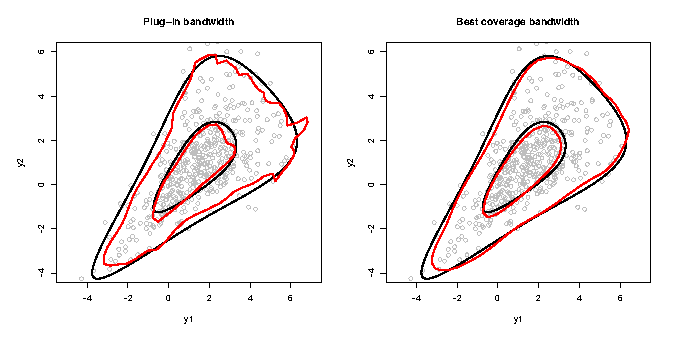
\includegraphics[width=0.90\textwidth]{Fig1.pdf}
	\caption{Estimated reference regions for plug-in and best coverage bandwidths for non-gaussian data. In black we represent true regions and in red the estimated ones for $\tau = 0.50, 0.95$. Best coverage bandwidth offers a smoother region than plug-in estimator.}
	\label{H}
\end{figure}


The selection of $\bf H$ is crucial to obtain a good estimation of $\varepsilon_{\tau}$. A natural option is to use a plug-in or cross-validation bandwidth estimator, as in a density estimation problem
\begin{equation}
\ \underset{\textbf{H} \in \mathcal{H}}{\operatorname{arg\min} } \textsf{E}(\iint \left(\hat{f}_\textbf{H}(\varepsilon_{1},\varepsilon_{2}) - f_\textbf{H}(\varepsilon_{1},\varepsilon_{2})^{(-i)} \right)^2 d\varepsilon_{1}d\varepsilon_{2} 
\label{CV}
\end{equation}
\noindent where $\hat{f}_\textbf{H}(\varepsilon_{1},\varepsilon_{2})^{-i}$ is the estimated bivariate density function without the i-th observation. However, as we seek for a probabilistic region (i.e. a region which contains a given percentage of the multivariate data), the following selection criteria based on the region coverage is proposed
\begin{equation}
\hat{\lambda} = \underset{\lambda}{\operatorname{arg\min} } \left|\left(n^{-1}\sum_{i=1}^n I \{(Y_{i1},Y_{i2})\in R^{(-i)}(\textbf{X}_i)\}\right) - \tau\right|
\label{CV1}
\end{equation}
\noindent where $\tau$ is the desired coverage and $\hat{R}_{\tau}^{(-i)}(X_i)$ is the estimated bivariate region without the i-th observation. Using this criteria the estimated region show a smoother contour and a coverage of the data points closer to the desired one $\tau$ (see Figure \ref{H}). Given the high computational cost of the regular proposed method in (\ref{CV}), a k-fold cross-validation scheme could be used instead. Moreover we simplify the minimization problem by considering $h_{11}=h_{22}$ and $h_{12}=0$.


\section{Overview of the package}

The \CRANpkg{refreg} package contains a set of functions for estimating a conditional reference, or uncertainty, region. Its working framework was designed so that people without a strong statistical background can use it. Indeed, only two functions need to be taken into account by the user: 1) the effects of the predictor variables on responses need to be estimated using the bivRegr function, a step that requires the user choose which variables may influence the region; 2) bivRegion needs to be applied to a bivRegr object so that the reference region can be estimated. 

The \code{bivRegr()} function has the following structure:

\begin{center}
\code{
	bivRegr(f = formulas, data = data)
}
\end{center}

The \code{f} argument contains a list of five R formulae corresponding to the additive predictors for the means, variances and correlation models shown in equation (1). Since \code{bivRegr()} uses \code{mgcv::gam()} internally, the user can estimate covariate linear and non-linear effects using \code{s()} operator. For instance:

\begin{example}
mu1 <- y1 ~ s(x1)
mu2 <- y2 ~ s(x1)
var1 <- ~ x2
var2 <- ~ x2
rho <- ~ s(x3)
	
formula = list(mu1,mu2,var1,var2,rho)
\end{example} 

\noindent assumes a smooth effect of \code{x1} on the response means, a parametric effect of \code{x2} on their variances, and a smooth effect of \code{x3} on the response correlation.

The \code{bivRegion()} function is designed for non-parametrically estimating a bivariate reference region:


\begin{center}
\code{bivRegion(object, tau = 0.95, bandwidth = "plug-in")}
\end{center}

The object may be a set of bivariate data points, or a \code{bivRegr} object, while tau defines the desired coverage(s) for the reference region, which might be a single value or a vector. Finally, ``bandwidth'' specifies the kernel bandwidth selection method. The user can chose between the plug-in, cross-validation, or the best coverage method (see equation (13)).
 

Additionally, we defined S3 methods for these two main functions. Specifically, associated with \code{bivRegr} we have
	

\begin{itemize}
\item \code{predict.bivRegr} and \code{plot.bivRegr}: to predict and depict additive models results for responses' means, variances, and their correlation.
\item \code{summary\_boot.bivRegr}: a function implementing the bootstrap inference for flexible additive models (see \eqref{boot}). This function results can be depicted by applying \code{plot.summary\_boot}. 
\end{itemize}

On the other hand, we defined the following S3 methods associated to \code{bivRegion}:

\begin{itemize}
\item  \code{summary.bivRegion}: this function evaluates the region performance on the healthy patients' sample.
\item \code{predict.bivRegion} and \code{plot.bivRegion}: these functions offer a prediction or a plot of conditional regions for a new dataset. If the argument \code{cond=FALSE} it evaluates the response values in the standardized scale. 
\end{itemize}
	
In addition, we define the functions \code{trivRegr}, \code{trivRegion} and \code{plot.trivRegion} as an extension of the aforementioned method for a trivariate response variable. Finally, our package also contains some inner functions as \code{ace} (for estimating variance, and correlation models), \code{Hcv} (it implements equation \eqref{CV1} method), and  \code{refcurve} (it implements an univariate location-scale model).

\section{Refreg in practice}

This section outlines the implemented functions of the proposed package in detail, and illustrates their use with real datasets. The first illustration is related to diabetes research, in which a reference region for the joint interpretation of two glycemia tests is calculated. In the second illustration, \CRANpkg{refreg} methodology is used to predict the concentrations of two air pollutants during a pollution episode. Finally, the extension of the method to higher dimensions is shown using real data.

\subsection{Case 1: Glycemic tests for diabetes diagnosis}

Diabetes is a chronic disease, the diagnosis of which is based on two glycemia tests: the fasting plasma glucose (FPG) and glycated hemoglobin (HbA1c)\citep{american20192} tests. The multivariate interpretation of FPG and HbA1c results is desirable for two reasons: i) the results of both tests are correlated in healthy patients \citep{aleyassine1980glycosylated}, ii) a miss-match between them may be indicative of a poorer prognosis \citep{kim2018hemoglobin}. Finally, it is well known that both test results are influenced by patient age \citep{davidson1979effect,pani2008effect}. 

The age-dependent reference region for the FPG and HbA1c tests was estimated using a sample of healthy subjects derived from the A-Estrada Glycation and Inflammation Study (AEGIS) (see \citep{gude2017glycemic}). A subset of this dataset is available in the package under the name ``AEGIS''.

This dataset comprised 1516 subjects and 7 variables:

\begin{itemize}
	\item id: an anonymous identifier for each subject.
	\item gender: a factor variable that indicates the subject's gender with levels ``male'', and ``female''.
	\item age: the subject's age.
	\item dm: a factor variable indicating a previous diabetes mellitus diagnosis with levels ``no'', and ``yes''.
	\item fpg: fasting plasma glucose concentration in mg/dL. 
	\item hba1c: the percentage of glycated hemoglobin. 
	\item fru: fructosamine plasma concentration.
\end{itemize}

Applying the \code{summary()} routine to the \code{aegis} dataset indicated 55\% of the subjects to be female, the mean age of all 1516 subjects to be 52 years (range 18-91), and that 187 subjects (12\%) had been previously diagnosed with diabetes.

\begin{example}
R> summary(aegis)
       id            gender         age          dm            fpg        
Min.   :   1.0   female:838   Min.   :18.00   no :1329   Min.   : 63.00  
1st Qu.: 379.8   male  :678   1st Qu.:39.00   yes: 187   1st Qu.: 82.00  
Median : 758.5                Median :52.00              Median : 89.00  
Mean   : 758.5                Mean   :52.58              Mean   : 94.51  
3rd Qu.:1137.2                3rd Qu.:67.00              3rd Qu.:100.00  
Max.   :1516.0                Max.   :91.00              Max.   :274.00  

hba1c             fru       
Min.   : 3.900   Min.   :119.0  
1st Qu.: 5.200   1st Qu.:225.0  
Median : 5.400   Median :254.0  
Mean   : 5.608   Mean   :262.2  
3rd Qu.: 5.700   3rd Qu.:284.0  
Max.   :10.200   Max.   :700.0  
\end{example}

To estimate the reference region, a subset of the patients not previously diagnosed with diabetes was define as \code{dm\_no}. This subset sample was deemed the healthy patient sample.

\begin{example}
R> dm_no = subset(aegis,aegis$dm == "no")
R> dm_yes = subset(aegis,aegis$dm == "yes")
\end{example}

To estimate the effect of age on the final region shape, the \code{bivRegr()} function was used. This function implements the estimation process of the bivariate location-scale:

\begin{example}
R> mu1 = fpg ~ s(age)
R> mu2 = hba1c ~ s(age)
R> var1 = ~ s(age)
R> var2 = ~ s(age)
R> rho = ~ s(age)
R> formula = list(mu1,mu2,var1,var2,rho)
\end{example}

The first and second formulae define the additive models for the mean values of both glycemia tests. The third and fourth define the additive models for test result variability. The last formula represents the additive model that comprises the effect of age on the correlation between the results of both glycemia tests. In addition to the model formulae list, a dataset including both the test results and subject's age must be supplied to \code{bivRegr()} as:


\begin{example}
R> fit = bivRegr(formula,data=dm_no)
\end{example}

\begin{figure}[!htb]
	\centering
	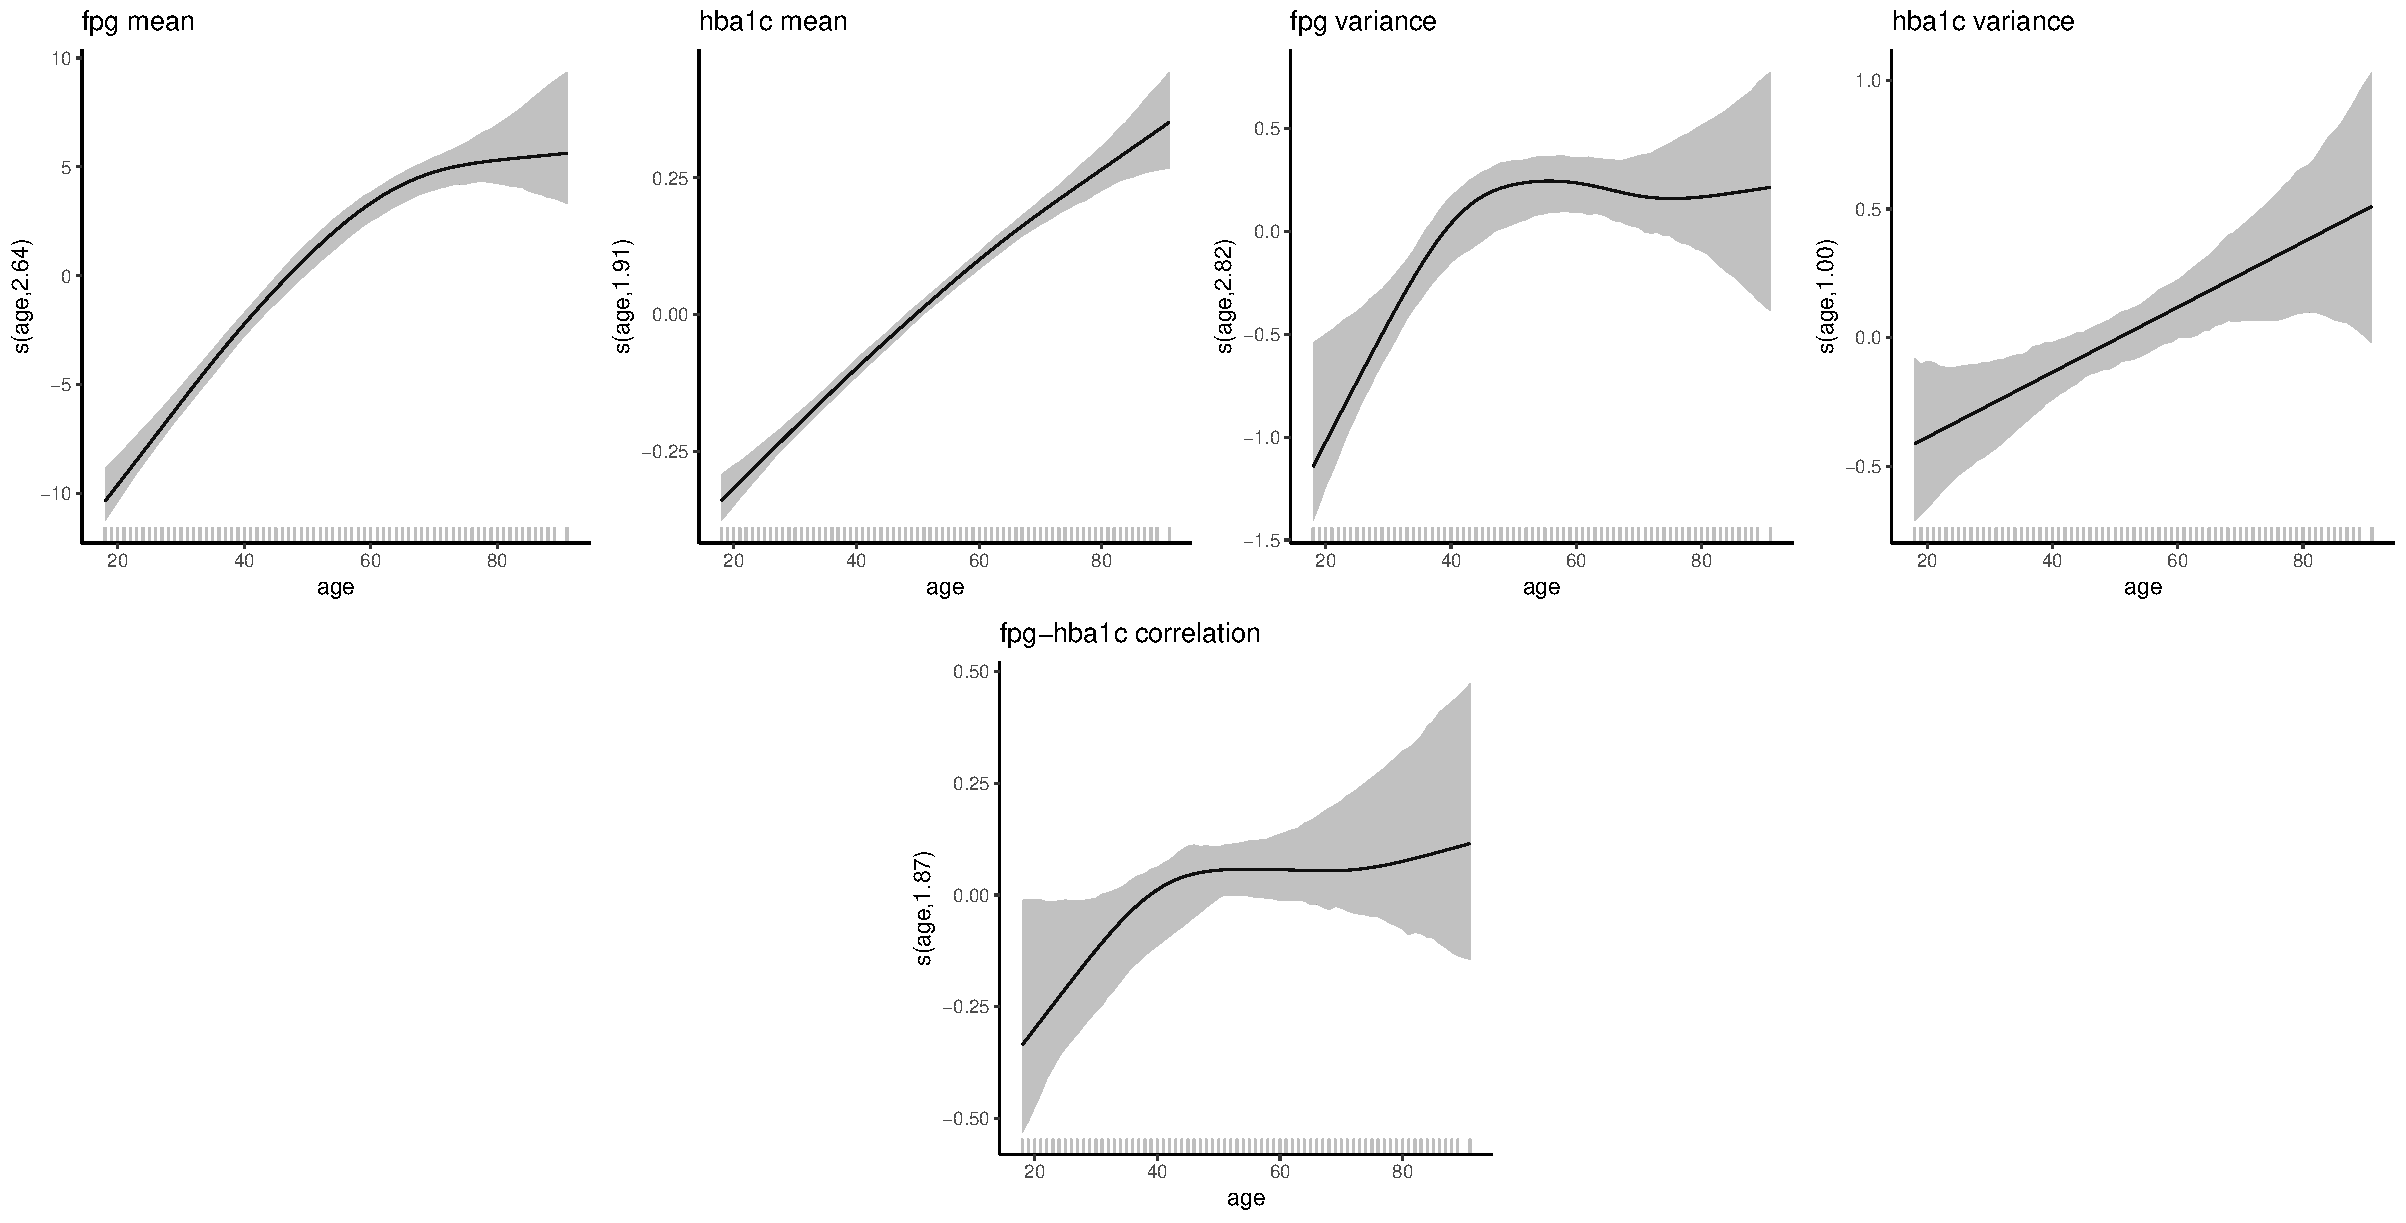
\includegraphics[width = \textwidth]{Fig2.pdf}
	\caption{Estimated effects of age on the FPG and HbA1c mean, variance models, and on their correlation. Output from \code{summary\_boot}, the shaded area is the 95\% pointwise confidence interval obtained by bootstrap resampling. The parameters of our bivariate response change with age.} 
	\label{effects}
\end{figure}


By applying the S3 method \code{plot()} to a \code{bivRegr} object, the estimated effects of covariates can be shown for each submodel. The argument eq= controls the model component to be represented (1 = FPG mean, 2 = HbA1c mean, 3 = FPG variance, 4 = HbA1c variance, and 5 = [FPG – HbA1c] correlation). Moreover, the function \code{summary\_boot()} may be applied to a \code{bivRegr} object to obtain the 95\% pointwise confidence interval for the estimated effects via bootstrapping:


\begin{example}
R> fit_boot = summary_boot(fit, B=250, parallel = TRUE )
R> plot(fit_boot,eq=1)
R> plot(fit_boot,eq=2)
R> plot(fit_boot,eq=3)
R> plot(fit_boot,eq=4)
R> plot(fit_boot,eq=5) 
\end{example}

Since bootstrap resampling (introduced in equation (\ref{boot})) is time consuming, the user can fix \code{parallel = TRUE} and run a parallelized computation. The parallel backend is registered using \CRANpkg{doParallel} \citep{doparallel}, and the parallel computation is performed by \CRANpkg{foreach} \citep{foreach}.




Figure \ref{effects} shows that the mean values of both glycemia markers increase almost linearly with age. FPG variance increases from 20 to 40 years, while the HbA1c variance increases linearly with age. Finally, the correlation between the FPG and HbA1c concentration seems to be stronger for older patients.


\begin{figure}[!htb]
	\centering
	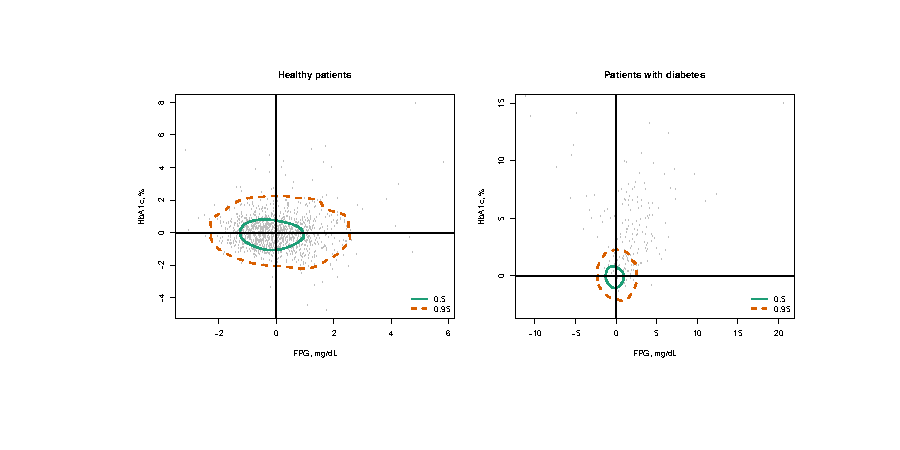
\includegraphics[width = \textwidth]{Fig3.pdf}
	\caption{Estimated region in the bivariate residuals scale for healthy patients (left), and patients with diabetes (right). Green contour represents the region for $\tau = 0.50$, while red dashed contour for $\tau = 0.95$.}
	\label{bivregion}
\end{figure}

Applying the function \code{bivRegion()} to a \code{bivRegr} object provides a bivariate region containing 100$\tau$\% of the model standardized residuals. This region is based on a bivariate kernel density estimator. The kernel bandwidth selection method may be chosen with the \code{H\_choice} argument. Here, the 90\%, 95\% and 97.5\% regions are obtained with the best coverage bandwidth selector (see equation \eqref{CV}):


\begin{example}
R> region = bivRegion(fit,tau=c(0.90,0.95,0.975),H_choice = "Hcov")
\end{example}

This region facilitates a multivariate interpretation of the glycemia test results. A patient whose results are ``normal'', for his/her age would see them fall inside this reference region, while a subject with ``abnormal'' results for his/her age would not. This interpretation is possible because the model residuals are centered around zero, show unit variance, no correlation, and they are independent of age. The user can check test results located outside the reference region using the \code{bivRegion} S3 method \code{plot}:


\begin{example}
R> par(mfrow = c(1, 2))
R> plot(region, xlab = "FPG, mg/dL", ylab = "HbA1c, \%",cond=T, newdata = 
 data.frame (age = c(20,30,40,50,60,70)),tau=0.95,reg.lwd=2, pch="*",col="grey")

R> plot(region,xlab = "FPG, mg/dL", ylab = "HbA1c, %",cond=T, newdata = 
   data.frame(age = c(20,60)),tau=c(0.50,0.95), reg.lwd=2, pch="*", col="grey")
\end{example}

Figure \ref{bivregion} shows the unconditional reference region for $\tau = 0.90, 0.95$ and $0.975$ for healthy patients, and those previously diagnosed with diabetes. Note that the \code{plot()} function argument 'newdata' allows the glycemia test values to be observed in the standardized residuals scale of the dataset for the patients with diabetes. As is clearly seen, most of healthy patients' results are located inside the reference region, while those recorded for diabetic patients are located outside.




A major advantage of this representation is that it allows clinicians new insights into the subject’s glycemia status. Indeed, those patients located outside the reference region may be classified into four groups: (I) individuals with high values for both tests (first quadrant); (II) those with discordant results, with high HbA1c concentrations and low/medium FPG (second quadrant); (III) individuals with low values for both tests (third quadrant); and (IV) individuals with low/medium HbA1c concentrations and high FPG values (fourth quadrant). This distinction might be useful for physicians. For instance, discordant results are probably due to an altered bloodstream protein glycation rate, a condition associated with a poorer prognosis. Patients located outside the standardized region may be also checked applying \code{summary()} to a \code{bivRegion} object:


\begin{example}
R> summary(region,tau = 0.95)
\end{example}

This R output presents patients located outside the standardized bivariate region for $\tau = 0.95$. Note that, in the full sample, patients with different ages were located outside the reference region. The glycemia tests results located outside the reference region are interesting from a clinical point of view. For example, the following were seen: a possible case of undiagnosed diabetes in a 20 year old patient (FPG = 99, HbA1c = 6.3); a 47 year old patient showing a high HbA1c value for his corresponding FPG result (FPG = 86, HbA1c =6); and a patient of 85 years in the opposite situation (FPG = 120, HbA1c = 5.7).


\begin{figure}[!htb]
	\centering
	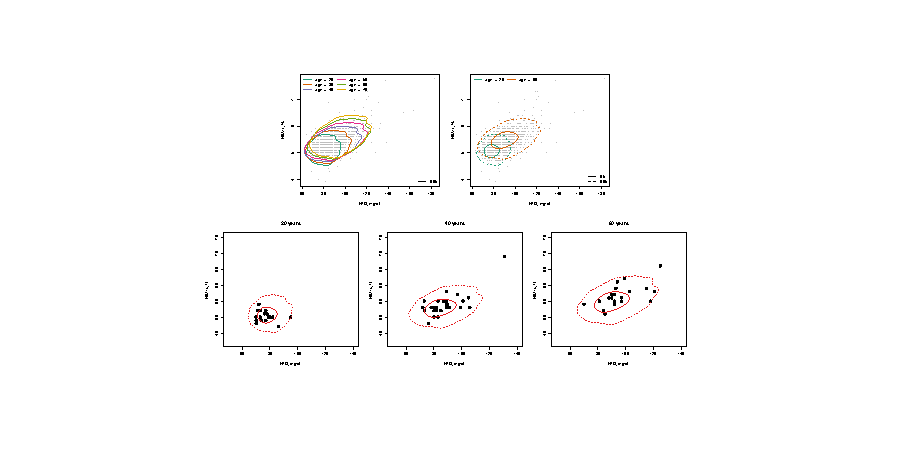
\includegraphics[width = \textwidth]{Fig4.pdf}
	\caption{Predicted reference regions for different ages. Solid line contour represents the reference region for $\tau = 0.50$, and the dashed line contour for $\tau = 0.95$. Toprow plots are depicted by \code{plot.bivRegion} function setting the arguments \code{cond=TRUE} and \code{add=FALSE} for several ages, and bottomrow ones with \code{cond=TRUE} and \code{add=TRUE} in a pre-existing plot. The estimated regions change with age and it describes the shape of the observed data points.}
\end{figure}

%
%\begin{example}
%$Values_out_of_reference_region_tau$Values_out_of_reference_region_tau$`Tau = 0.95`
%$Values_out_of_reference_region_tau$`Tau = 0.95`$`Both high`
%     fpg hba1c age   fpg-res hba1c-res
%52   118   6.2  64 1.3337154 1.8577269
%55    98   6.0  32 0.5536627 2.6946600
%71    99   6.3  23 1.6099530 4.3388638
%220  125   6.1  50 2.1279498 2.1295106
%264  122   5.9  76 2.3828303 0.6623911
%292  117   5.6  45 2.3856741 0.7420889
%377  121   7.3  84 0.1625022 4.0145448
%456  100   5.2  25 2.5656719 0.1628346
%525  125   5.4  36 4.1469217 0.4228002
%623  117   6.7  59 0.3140963 3.5323795
%731   94   5.7  22 1.5781388 2.1622899
%
%$Values_out_of_reference_region_tau$`Tau = 0.95`$`fpg low and hba1c high`
%     fpg   hba1c age     fpg-res hba1c-res
%134  105 6.30000  52 -0.15701652 2.6609786
%391   73 5.90000  62 -2.49473184 1.0605236
%699  109 7.00000  70 -0.73439258 3.8605528
%1308 102 6.40000  38 -0.20052254 3.7283590
%1334  69 5.60753  25 -2.17761431 1.6595322
%1375  86 6.00000  47 -1.40191901 1.9465450
%1419  85 6.90000  43 -3.09131126 5.0801213
%1425  69 5.80000  58 -2.69314308 0.8989238
%
%
%$Values_out_of_reference_region_tau$`Tau = 0.95`$`Both low`
%     fpg hba1c age    fpg-res hba1c-res
%144  75   4.6  62 -0.1057527 -2.719202
%658  69   4.3  35 -0.2285157 -3.330018
%
%$Values_out_of_reference_region_tau$`Tau = 0.95`$`fpg high and hba1c low`
%      fpg hba1c age   fpg-res   hba1c-res
%19    85   4.7  51 0.8411861 -2.27800030
%36    82   3.9  61 1.7722484 -4.75817426
%123  129   5.0  44 4.7020255 -1.17441005
%167   88   4.7  69 0.8967447 -2.49034872
%238   85   4.4  55 1.3159600 -3.25155962
%256   96   4.7  49 1.9223660 -2.24425172
%486  120   5.7  85 2.5829613 -0.05351398
%574  101   4.9  78 1.8840723 -2.01508017
%1263  86   4.3  21 1.6304780 -3.05526652
%1447  95   5.0  20 2.5475005 -0.37916145
%\end{example}

The use of this region in combination with the results of the bivariate location-scale model allow the conditional reference regions to be obtained. The user can visualize these regions using the \code{bivRegion} S3 method \code{plot()}, setting \code{cond = TRUE} as follows:

\begin{example}
R> plot(region, xlab = "FPG, mg/dL", ylab = "HbA1c, %",cond=T, newdata = data.frame(age =
   c(20,30,40,50,60,70)),tau=0.95,reg.lwd=2, pch="*",col="grey")

R> plot(region,xlab = "FPG, mg/dL", ylab = "HbA1c, %",cond=T, newdata = data.frame(age =
   c(20,60)),tau=c(0.50,0.95),reg.lwd=2, pch="*",col="grey")	
\end{example}


In addition, the region may be represented in a pre-existing plot if the \code{plot} function argument \code{add} is equal to \code{TRUE} as in the following code:

\begin{example}
R> plot(dm_no[dm_no$age==40,"fpg"],dm_no[dm_no$age==40,"hba1c"],main="40 years",
   xlim=c(50,140), ylim=c(4.2,7.5),xlab = "FPG, mg/dL", ylab = "HbA1c, %", pch=20,cex=2)
R> plot(region,cond=T,newdata = data.frame(age = 40),add=T,legend=F, tau=c(0.50,0.95),
   reg.lty=c(1,2))

R> plot(dm_no[dm_no$age==60,"fpg"],dm_no[dm_no$age==60,"hba1c"],main="60 years", 
   xlim=c(50,140), ylim=c(4.2,7.5),xlab = "FPG, mg/dL", ylab = "HbA1c, %", pch=20,cex=2)
R> plot(region,cond=T,newdata = data.frame(age = 60),add=T,legend=F, tau=c(0.50,0.95),
   reg.lty=c(1,2))
\end{example}

In Figure 4, the bivariate reference region is shown for several ages. Note that the regions shift towards the upper right corner and expand as age increase. This agrees with the non-linear effect of age on the expected means and variability of both markers. The conditional region coverage and the performance of the methodology have already been assessed \citep{statmed}.


\subsubsection{Extension of case 1, conditional reference region for a trivariate response}

This section provides an example of how the method proposed in equation (3) might be extended to more than two dimensions. This section is intended to provide a proof of concept rather than a formal statistical proposal. For a trivariate variable ($Y_1, Y_2, Y_3$) the following model can be assumed:
\begin{equation}
	\left( {
		\begin{tabular} {c}
			$Y_1$ \\
			$Y_2$\\
			$Y_3$\
		\end{tabular}
	}\right) = \left( {
		\begin{tabular} {c}
			$\mu_1(\textbf{X})$ \\
			$\mu_2(\textbf{X})$\\
			$\mu_3(\textbf{X})$\
		\end{tabular}
	}\right)
	+  \boldsymbol{\Sigma}^{1/2} (\textbf{X})
	\left( {
		\begin{tabular} {c}
			$\varepsilon_1$ \\
			$\varepsilon_2$\\
			$\varepsilon_3$\\
		\end{tabular}
	}\right)
	\label{mod3}
\end{equation}
\noindent
where $\{\mu_r(\textbf{X})\}_{r=1}^3$ represents the conditional means of each response, and $\boldsymbol{\Sigma}^{1/2} (\textbf{X})$ the Cholesky decomposition of the variance-covariance matrix
\begin{equation}
	\boldsymbol{\Sigma} (\textbf{X})=\left({
		\begin{tabular} {ccc}
			$\sigma_1^2 (\textbf{X})$  &  $ \sigma_{21} (\textbf{X})$&  $ \sigma_{31} (\textbf{X})$\\
			$\sigma_{12} (\textbf{X})$ & $\sigma_2^2 (\textbf{X})$&  $ \sigma_{23} (\textbf{X})$  \\
			$\sigma_{13} (\textbf{X})$ & $\sigma_{32} (\textbf{X})$ &  $ \sigma_3^2 (\textbf{X})$ \\
	\end{tabular}}\right)
\end{equation}
In the trivariate case, the estimated variance-covariance matrix can be non-positive-definite. Thus, $\hat{\boldsymbol{\Sigma}}$ is modified by applying the unweighted bending method of \cite{schaeffer2014making} as implemented in the \CRANpkg{mbend} R package \citep{nilforooshan2020mbend}.




Following equation (\ref{mod3}), a trivariate reference region may be estimated as:
\begin{equation}
	R_{\tau}(\textbf{X})
	=
	\left( {
		\begin{tabular} {c}
			$\mu_1(\textbf{X})$ \\
			$\mu_2(\textbf{X})$ \\
			$\mu_3(\textbf{X})$ 
			\
		\end{tabular}
	}\right)
	+ 
	\boldsymbol{\Sigma}^{1/2} (\textbf{X}) \varepsilon_{\tau}
\end{equation} 
\noindent where $\varepsilon_{\tau}$ is the unconditionally probabilistic region for the errors $(\varepsilon_1,\varepsilon_2,\varepsilon_{3})$ as 
\begin{equation}
	\varepsilon_{\tau} (k) = \{(\varepsilon_1,\varepsilon_2,\varepsilon_{3}) \in{\mathbb{R}}^3 | f(\varepsilon_1,\varepsilon_2,\varepsilon_{3}) \leq k\}
	\label{rexion_3}
\end{equation}
\noindent
$f$ being the density function of the trivariate residuals  $(\varepsilon_1,\varepsilon_2,\varepsilon_3)$ and  $k$ is the $\tau-$quantile of $f(\varepsilon_1,\varepsilon_2,\varepsilon_3)$. 

Using this model, the application of the methodology for diabetes diagnosis can be extended by incorporating an additional glycemia test. This extension is justified since other glycated proteins are routinely monitored in diabetes control besides FPG and HbA1c. For instance, in conditions that determine alterations in hemoglobin metabolism (e.g., anemia or kidney disease), fructosamine (Fr) is frequently used as an additional marker. Nevertheless, the translation of Fr into average glucose levels is not as clear as for HbA1c, and discordances are often encountered between the Fr and HbA1c results. In addition, agreement among these glycemia markers can be affected by factors such as patient age.

\begin{figure}[!htb]
	\centering
	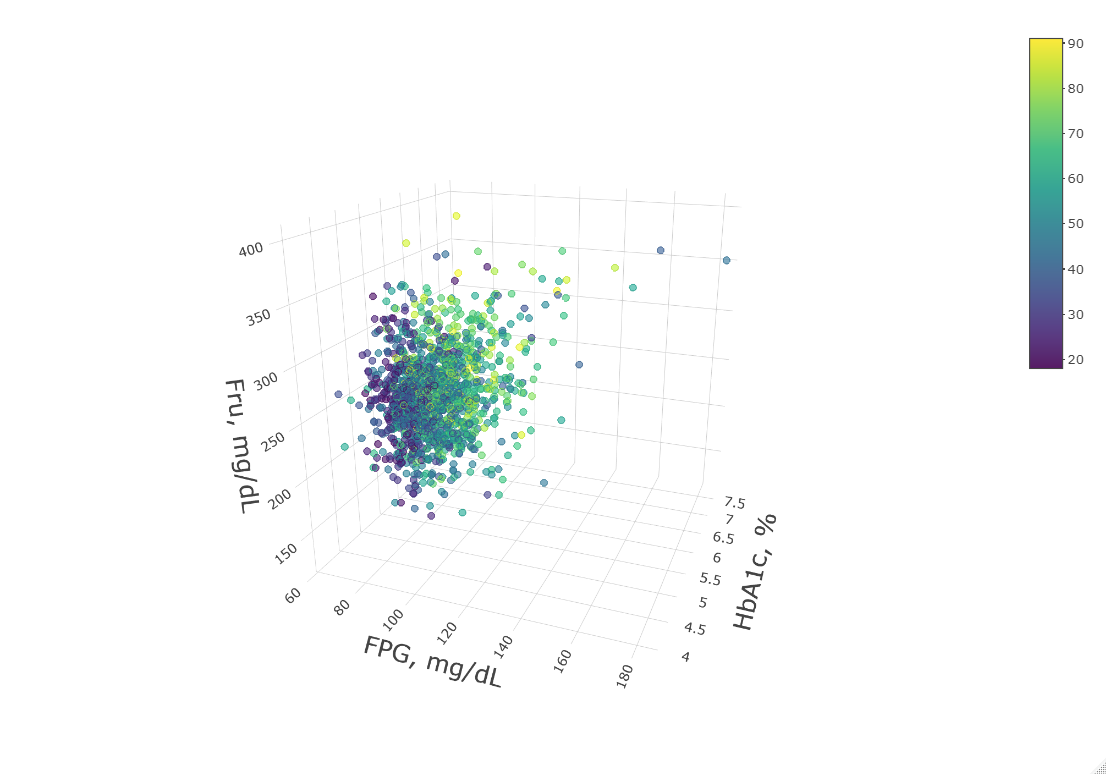
\includegraphics[width=0.49\textwidth]{Fig5.1.png}
	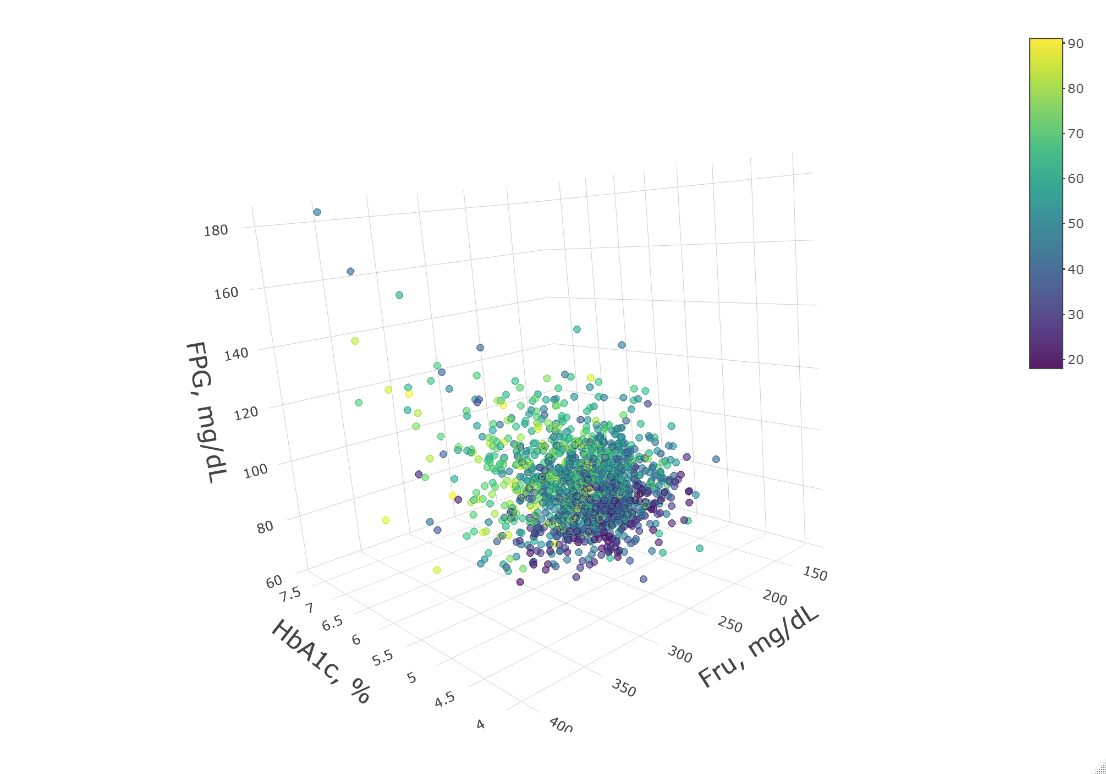
\includegraphics[width=0.49\textwidth]{Fig5.2.png}
	\caption{Scatter plot for three glycemic markers (fasting plasma glucose, glycated hemoglobin and fructosamine), with colour scale depending on age. The joint values of these glycemic markers seems to change with age, i.e., higher values are observed at higher ages. A trivariate and age-dependent reference region is desirable.}
	\label{3d}
\end{figure}

\begin{figure}[!htb]
	\centering
	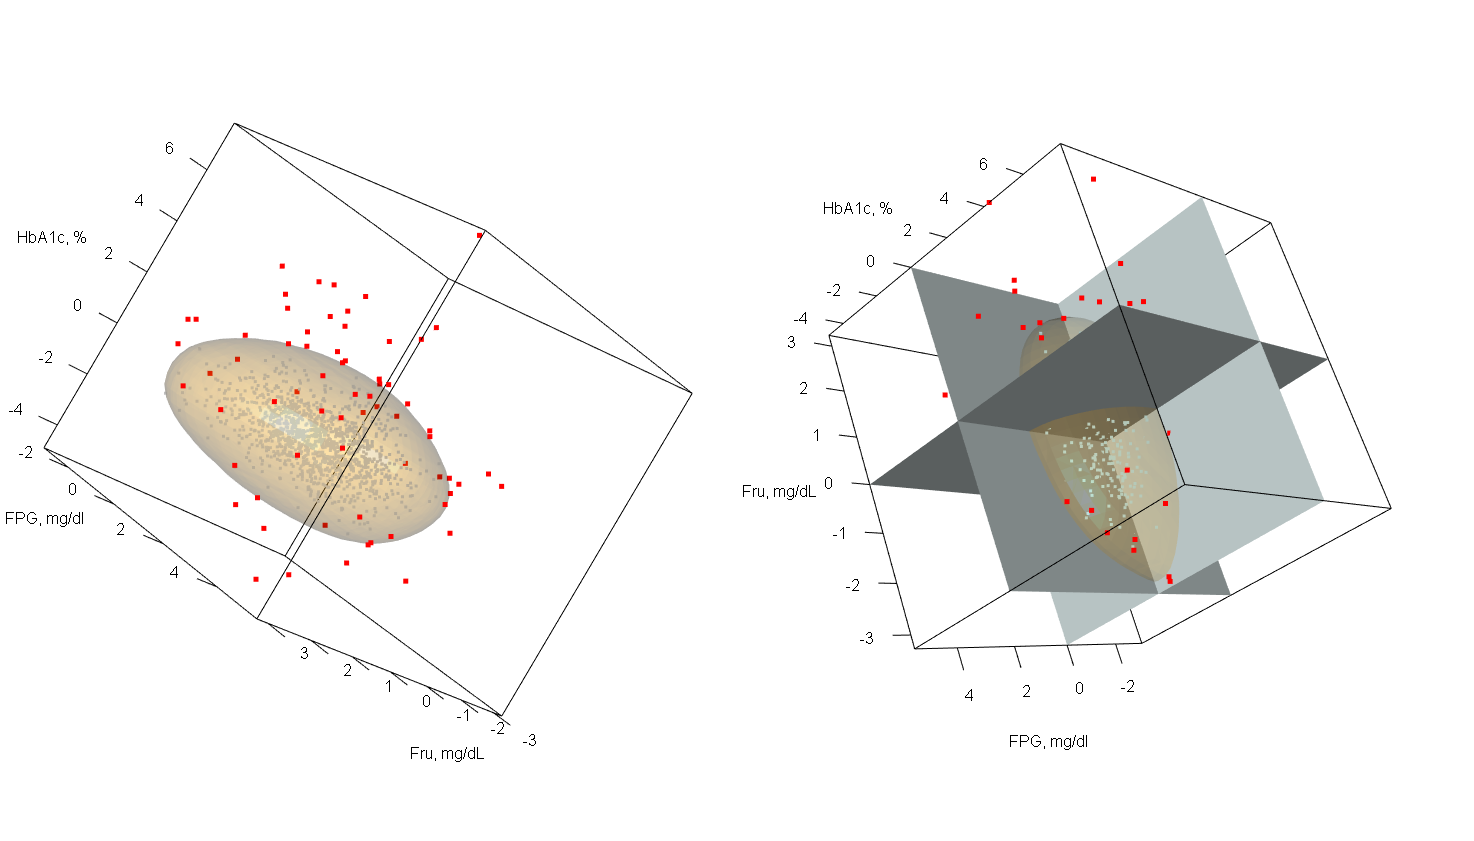
\includegraphics[width=0.8\textwidth]{Fig6.1.png}
	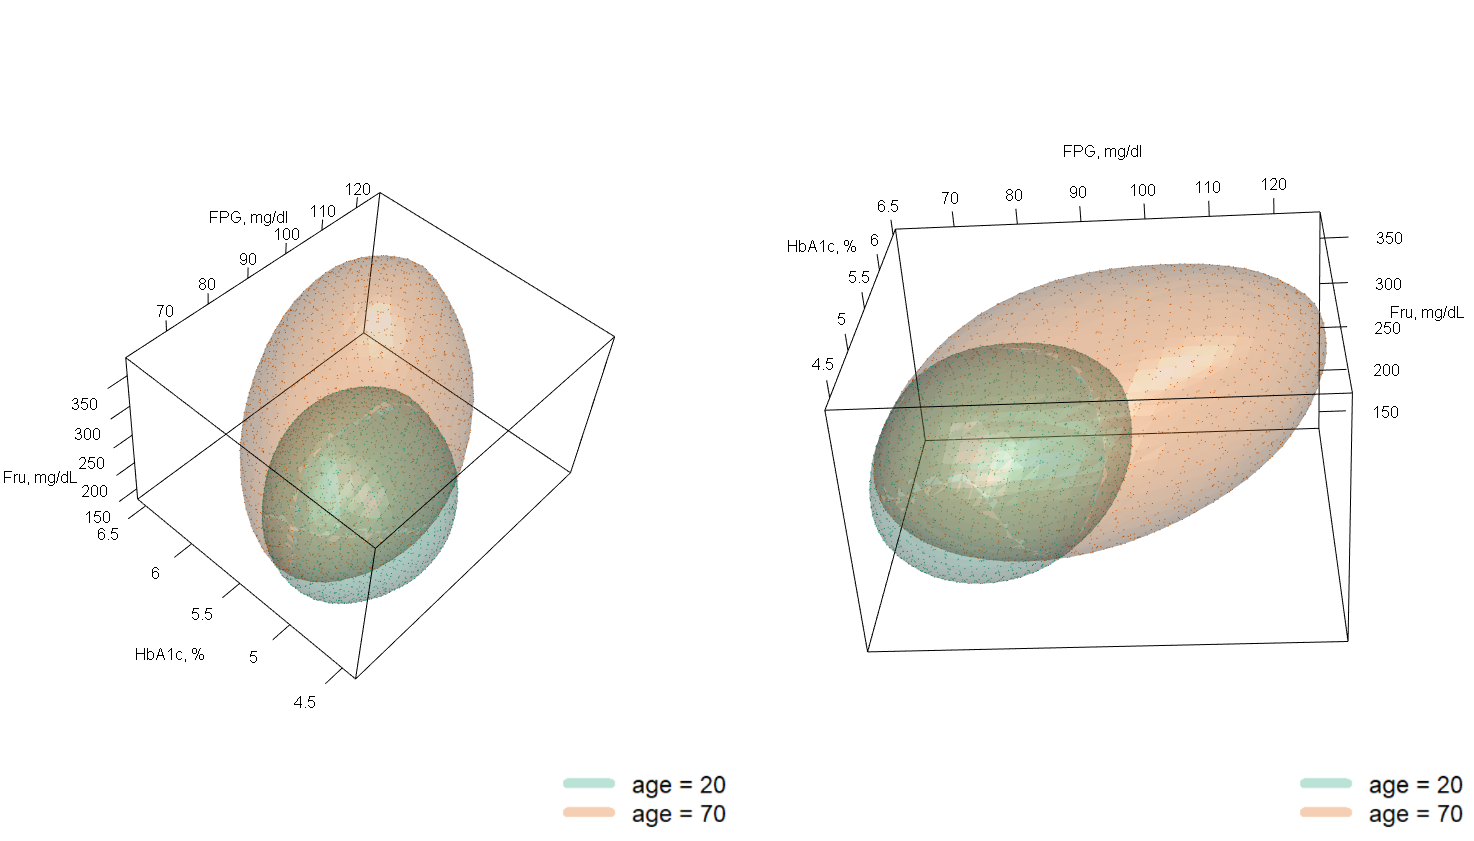
\includegraphics[width=0.8\textwidth]{Fig6.2.png}
	\caption{Standardized reference region (toprow plots), and conditional reference region (bottomrow plots), for three glycemic tests. Red points represent the trivariate values located outside the reference region after adjusting by age. The grey panels define eight octanes -- each one with a different clinical profile. The trivariate reference region for these markers changes with age.}
	\label{triv_res}
\end{figure}

Figure \ref{3d} show the FPG, HbA1c and Fr results for the AEGIS sample. As can be seen, the values recorded for these tests correlate with one another, showing a complex multivariate distribution. Moreover, it can be appreciated how their multivariate distribution changes with age. To estimate a trivariate reference region for these markers, taking into account patient age, the \code{trivRegr()} function was used. This function is an extension of \code{bivRegr()} to the trivariate setting. The usage of both functions is similar, but additional additive predictors must be defined for the means vector and variance-covariance matrix.





\begin{example}
R> dm_no = subset(aegis,aegis$dm == "no")
R> mu1 = fpg ~ s(age)
R> mu2 = hba1c ~ s(age)
R> mu3 = fru ~ s(age)
	
R> var1 = ~ s(age)
R> var2 = ~ s(age)
R> var3 = ~ s(age)
	
R> rho12 = ~ s(age)
R> rho13 = ~ s(age)
R> rho23 = ~ s(age)
	
R> formula = list(mu1,mu2,mu3,var1,var2,var3,rho12,rho13,rho23)
R> fit = trivRegr(formula,data=dm\_no)
\end{example}


As in the bivariate estimation, the \code{trivRegion} function is applied to a \code{trivRegr} object. Here, the method was implemented only for a single $\tau$ (the kernel density bandwidth selection was not formally tested). The \code{plot()} method implemented for the \code{trivRegion} object can be used to interactively check the trivariate standardized and conditional reference regions:


\begin{example}
R> region = trivRegion(fit,tau=0.95)
	
R> plot(region,planes = F,size=5, col="red", incol = "grey",xlab="FPG, mg/dl", 
   ylab="HbA1c, \%", zlab="Fru, mg/dL")
R> plot(region,planes = T,size=5,col="red",incol = "grey",xlab="FPG, mg/dl",
   ylab="HbA1c, \%", zlab="Fru, mg/dL")
R> plot(region,cond=T,newdata=data.frame(age=c(20,70)), xlab="FPG, mg/dl",
   ylab="HbA1c, \%", zlab="Fru, mg/dL", legend=T)
\end{example}

In Figure \ref{triv_res} the trivariate standardized and conditional reference regions are shown for different angles. The model residuals are centered around zero, with variance zero, and zero linear correlation. The region contains the 94.96\% of the patients. In the trivariate setting, a patient may be located outside the region for different reasons. Indeed, if \code{plot()} argument \code{panels=T}, eight reasons exist for why a patient is located outside the reference region (explaining each situation goes beyond the scope of the present work). The conditional reference region may be produced for different ages by setting the \code{cond = T}, and providing new age values in \code{newdata}.

\subsection{Case 2: beyond the medical research – Joint prediction of SO2 and NOx pollutants}

This section illustrates how \CRANpkg{refreg} methodology can be used in fields other than laboratory medicine. It is here shown how an uncertainty region useful for the joint forecasting of the concentration of two air pollutants ($SO_2$ and $NO_x$) can be derived using the \code{bivRegr} and \code{bivRegion} functions. The following example estimates which joint $SO_2$ and $NO_x$ values are more likely in the course of a pollution episode. The data, which are contained in the package, were obtained from the surroundings of the a coal-fire power station in the northern Spain. Current Spanish legislation places a limit on the mean of 24 successive determinations of pollution concentration taken at 5 minute intervals in the neighborhood of potential point sources of pollution. Thus, access was available to historical concentrations of both air pollutants over a year, as well as several records of pollution episodes.

Given the historical concentrations of both pollutants (contained in the \code{pollution} dataset), we aimed to predict the $SO_2$ and $NO_x$ concentrations during a specific pollution episode (contained in the \code{pollution\_episode} dataset) 30 minutes in advance. As can be seen in the following R output, both datasets have a similar structure, SO2 and Nox are the current concentrations of both pollutants, while the remaining columns represent their concentrations in the previous 30, 45, and 60 minutes.

\begin{figure}[!htb]
	\centering
	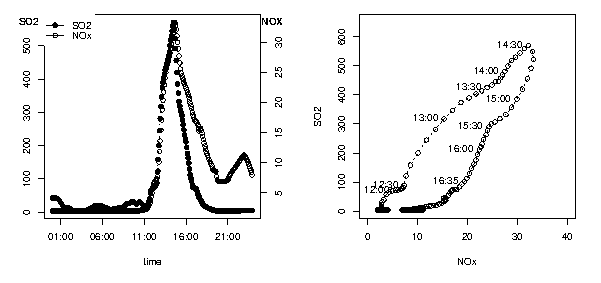
\includegraphics[width = 0.85\textwidth]{Fig7.pdf}
	\caption{Two different representations of a pollution incident for $SO_2$ and $NO_x$. Left plot represent the pollution episode in the univariate scale, and rigth plot in a bivariate scale. SO$_2$ and NO$_x$ pollution episodes are associated.}
	\label{episode}
\end{figure}




\begin{example}
R > head(pollution[,1:9])
                Date      So2   Nox   So2_0  Nox_0 So2_1  Nox_1 So2_2  Nox_2
316  2003-02-07 16:15:00  38.38  2.38  73.50  3.21  76.79  3.38  81.92  3.54
1865 2003-05-07 03:10:00   3.00  3.67   3.00  3.33   3.00  3.33   3.00  3.33
1383 2003-04-04 01:35:00 256.50 11.17 293.71  8.96 294.54  8.33 285.29  7.71
3262 2003-07-09 14:35:00 225.29 17.04 104.67  7.67  84.33  6.29  64.67  4.67
1191 2003-03-30 13:55:00  42.33  4.12  80.21  4.96  84.38  5.00  88.33  5.00
3065 2003-07-04 11:50:00 145.83  8.58  99.12  5.71  83.83  5.25  70.92  4.83
	
R > head(pollution_episode[,1:9])
                Date  So2  Nox So2_0 Nox_0 So2_1 Nox_1 So2_2 Nox_2
1 2003-05-09 00:00:00 3.08 4.12  3.08  4.50  3.08  4.46  3.08  4.38
2 2003-05-09 00:05:00 3.08 4.12  3.08  4.46  3.08  4.50  3.08  4.46
3 2003-05-09 00:10:00 3.08 4.12  3.08  4.38  3.08  4.46  3.08  4.50
4 2003-05-09 00:15:00 3.08 4.12  3.08  4.29  3.08  4.38  3.08  4.46
5 2003-05-09 00:20:00 3.08 4.12  3.08  4.21  3.08  4.29  3.08  4.38
6 2003-05-09 00:25:00 3.08 4.12  3.08  4.12  3.08  4.21  3.08  4.29
\end{example}


\begin{figure}[!htb]
	\centering
	%	\includegraphics[width = \textwidth]{PredEpisodioBiv.eps}
	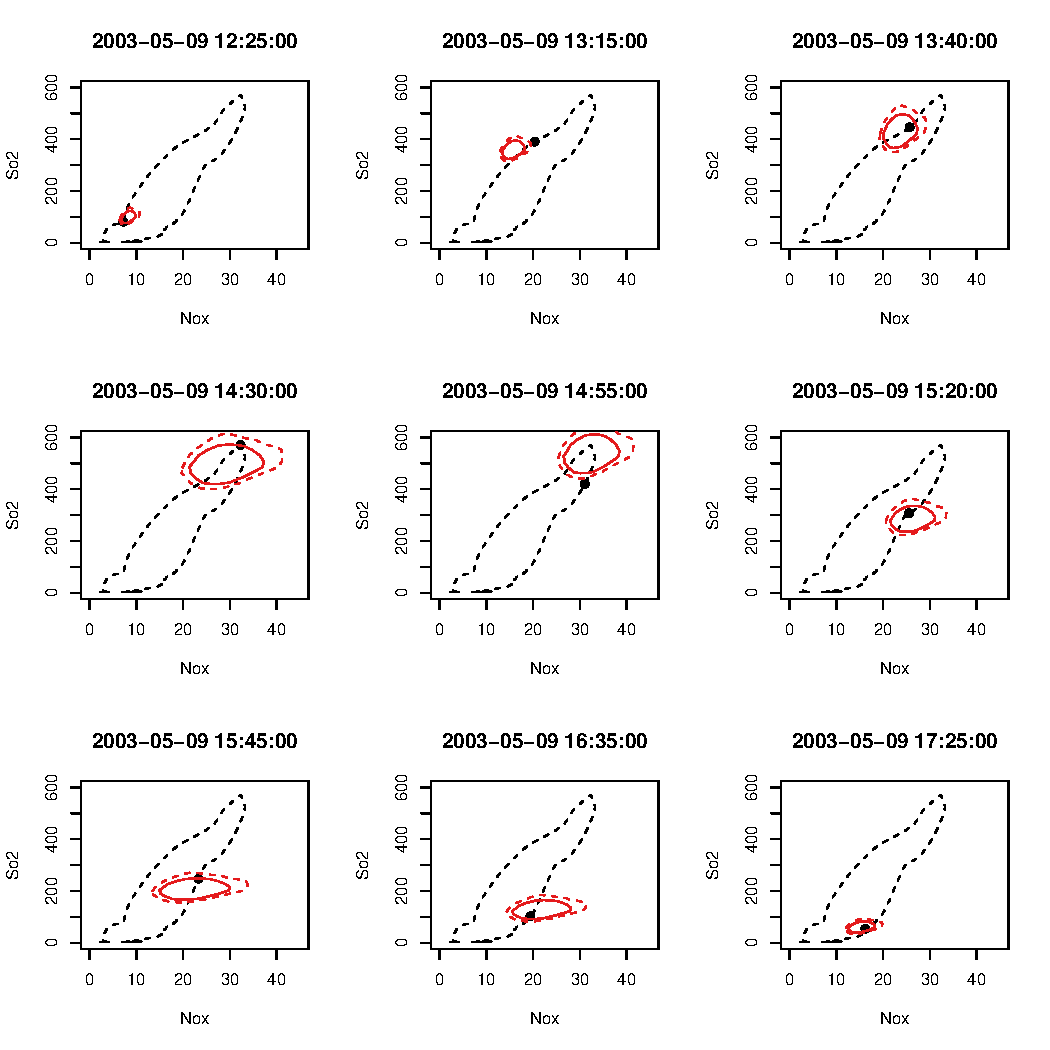
\includegraphics[width = \textwidth]{Fig8.pdf}
	\caption{Estimated bivariate uncertainty region for a pollution episode. Black dashed line represents the pollution episode evolution, solid black point the observed value, and red contours the predicted uncertainty region for $\tau = 0.95$ (red solid contour) and $\tau = 0.975$ (red dashed contour).}
	\label{pred_pol}
\end{figure}

Figure \ref{episode} shows the course of the pollution episode under prediction. In the left plot the $SO_2$ and $NO_x$ concentrations over time are represented by solid and open circles, respectively. Each point in the right plot of this figure shows the concentration of both pollutants at a specific instant in time. It can be can seen how, during a pollution episode, the concentration of both pollutants increases to a peak, and then returns slowly back to lower values. $NO_x$ increases in a manner similar to the $SO_2$, but its decrease is slower. Both representations show an evident correlation between the concentration of these air pollutants. To monitor this pollution episode, the historical records from the power plant were used, and $NO_x$ levels made dependent on their previous values (30, and 60, minutes before; $NO_{x_0}$, and $NO_{x_2}$). Similarly, the $SO_2$ concentration was made dependent on its prior concentration ($So2_0$, $So2_2$). Finally, the correlation between both was made dependent on the previous observation for both air pollutants ($Nox_0$, $So2_0$):


\begin{example}
R> mu1 = Nox~s(Nox_0)+s(Nox_2)
R> mu2 = So2~s(So2_0)+s(So2_2)
R> var1 = ~s(Nox_0)+s(Nox_2)
R> var2 = ~s(So2_0)+s(So2_2)
R> rho = ~s(Nox_0)+s(So2_0)
R> f = list(mu1,mu2,var1,var2,rho)

R> fit = bivRegr(f,data=pollution)
R> region = bivRegion(fit,tau=c(0.950,0.975),shape=10)
\end{example}

In the previous code example, the reference region was estimated for $\tau=0.95, 0.975$ for the model-standardized residuals. A pollution episode can then be forecasted by predicting the uncertainty regions based on the values provided by the \code{pollution\_episode} dataset. Note, that one dataset is used to fit the model, and another when making predictions. The observed $SO_2$ and $NO_x$ concentrations during the pollution episode are shown in Figure \ref{pred_pol} along with the predicted probabilistic regions. Each plot corresponds to a different instant in time, and to different pollution episode states. The upper right-hand side shows the beginning of the pollution episode, the bottom left plot shows its ending. The region's shape changes over time, anticipating reasonably well the evolution of the pollution episode. The size of the region becomes larger as the pollution peak is approached, and then gradually becomes smaller. This is to be expected since the maximum corresponds to a transition between the increase and decrease of the concentrations of both pollutants, a situation that involves more uncertainty. Moreover, at the end of the pollution episode, the region is higher on the X axis, which corresponds to greater uncertainty for the Nox prediction. As commented above, this might be explained in that the $NO_x$ concentration decreases more slowly than the $SO_2$ concentration.


\begin{example}
par(mfrow=c(3,3))
for(k in c(150, 160, 165, 175, 180, 185, 190, 200,210)){
	plot(pollution_episode[,3:2],type="l",lty=2,ylim=c(0,600),xlim=c(0,45),
	main=pollution_episode[k,1])
	points(pollution_episode[k,3:2],col="black",pch=19)
	plot(region, cond = T, newdata = pollution_episode[k,], add = T,
	tau=c(0.95, 0.975),legend=F)
}
\end{example}


\section{Concluding remarks}

This paper discusses the R implementation of a newly developed method for estimating conditional reference regions. The method was originally designed for bivariate responses to provide a joint interpretation of two glycemia markers. However, as shown with real data, the proposed package can be used in other fields, and its extension to three dimensions is feasible. The proposed package is useful in the definition of conditional reference regions for continuous diagnostic tests. Few MVRs applications are used in practice, yet they have been shown clinically valuable in the treatment of patients with cancer  \citep{mattsson2008multidimensional}, cardiovascular disease \citep{selmeryd2018derivation} and endocrine problems \citep{hoermann2016derivation}. Given the simplicity with which \CRANpkg{refreg} can be used, and its having no parametric restrictions, it is hoped it might enhance the use of MVRs.

The definition of a region characterizing the central part of a multivariate distribution may be of great interest in other fields. For instance, in quality control studies, multivariate control charts are commonly used when two or more attributes of a product, or process, require evaluation \citep{fuchs1998multivariate}. Analogously to medical MVRs, this multivariate analysis is currently performed assuming a Gaussian distribution. Thus, the \CRANpkg{refreg} R package may help provide for better quality surveillance of medical conditions, environmental problems and even industrial processes that are monitored by the measurement of more than one variable.

Future versions of our package will look forward to extending our model for continuous responses of dimension higher than three. Such reference region would require a kernel density estimator for high dimension applications \citep{kdevine}. To the best of our knowledge, the estimated region is not easy to visualize for scales larger than three. Although, we might identify and visualize the multivariate values located inside or outside the region using parallel coordinate plots, or the interactive visualization methods as the implemented in the \CRANpkg{tourr} package \citep{wickham2011tourr}.

\section{Acknowledgements}

Óscar Lado-Baleato is funded by a pre-doctoral grant (ED481A-2018) from the Galician Government (Plan I2C)-Xunta de Galicia. This study was also supported by grants from the Carlos III Institute of Health (Instituto de Salud Carlos III-ISCIII/PI20/01069/Co-funded by European Union), the Network for Research on Chronicity, Primary Care, and Health Promotion (Instituto de Salud Carlos III-ISCIII/RD21/0016/0022/Co-funded by European Union), and the Galician Innovation Agency-Competitive Benchmark Groups (GAIN-GRC/IN607A/2021/02/Xunta de Galicia). This article was developed under the project MTM2017-83513-R, cofinanced by the Ministry of Economy and Competitiveness (SPAIN) and by the European Regional Development Fund (FEDER). The work was also supported by the project ED431C 2020/20, approved within the framework of the Competitive Research Unit Consolidation Programme (2020), Xunta de Galicia. Work supported by the Grant PID2020-118101GB-I00, Ministerio de Ciencia e Innovación (MCIN/ AEI /10.13039/501100011033).  


\bibliography{Lado_Baleato_et_al}

\address{Óscar Lado-Baleato\\
  Department of Statistics, Mathematical Analysis, and Optimization, Universidade de Santiago de Compostela, Galicia, Spain.\\
  Medicine Colleague, Rúa San Francisco, Santiago de Compostela.\\
  Galicia, Spain\\
  (https://orcid.org/0000-0001-9592-4879)\\
  \email{oscarlado.baleato@usc.es}}

\address{Javier Roca-Pardiñas\\
	Galician Center for Mathematical Research and Technology (CITMAga) \&
  Statistical Inference, Decision and Operations Research, Universidade de  Vigo.\\
  Rúa do Conde de Torrecedeira, 86, 36310 Vigo, Pontevedra.\\
   Galicia, Spain\\
  \email{roca@uvigo.com}}

\address{Carmen Cadarso-Suárez\\
	Galician Center for Mathematical Research and Technology (CITMAga) \&
 Department of Statistics, Mathematical Analysis, and Optimization, Universidade de Santiago de Compostela, Galicia, Spain.\\
Medicine Colleague, Rúa San Francisco, Santiago de Compostela.\\
 Galicia, Spain\\
  \email{carmen.cadarso@usc.es}}

\address{Francisco Gude\\
	Clinical Epidemiology Unit, Complexo Hospitalario de Santiago de Compostela.\\
	Rúa da Choupana, s/n, 15706 Santiago de Compostela, A Coruña\\
	 Galicia, Spain\\
	\email{francisco.gude.sampedro@sergas.es}}

